\section{PDEs in rectangular coordinates}

In this section, we will consider the separation of variables for more general equations in rectangular coordinates, possibly with variable coefficients and more general boundary conditions. 

\subsection{Boundary conditions for general PDEs}


\subsubsection{Dirichlet, Neumann and Robin boundary conditions}

In the ODE class, we have learned the following boundary value problem
\begin{equation}\label{eq.ODE_boundary}
    \begin{split}
        &u'' = 1, \qquad x\in [0, 1]
        \\
        &u(0) = 0,\quad u(1) = 0.
    \end{split}
\end{equation}
where we prescribe a condition for every point on the boundary of the domain $[0, 1]$. (The boundary is $0$ and $1$.) If we miss any of these conditions, we cannot get a unique solution. 

For example, if we remove the condition $u(1) = 0$, then we get solution $u(x) = \frac{1}{2}x^2 + Cx$, which contains an undetermined constant $C$.

Given a PDE defined on a domain $R$, we must also prescribe the boundary condition on $\partial R$ to obtain a unique solution.

\begin{figure}[H]
    \begin{tikzpicture}
        \node at (0, 0) {
            \scalebox{0.2}{      
                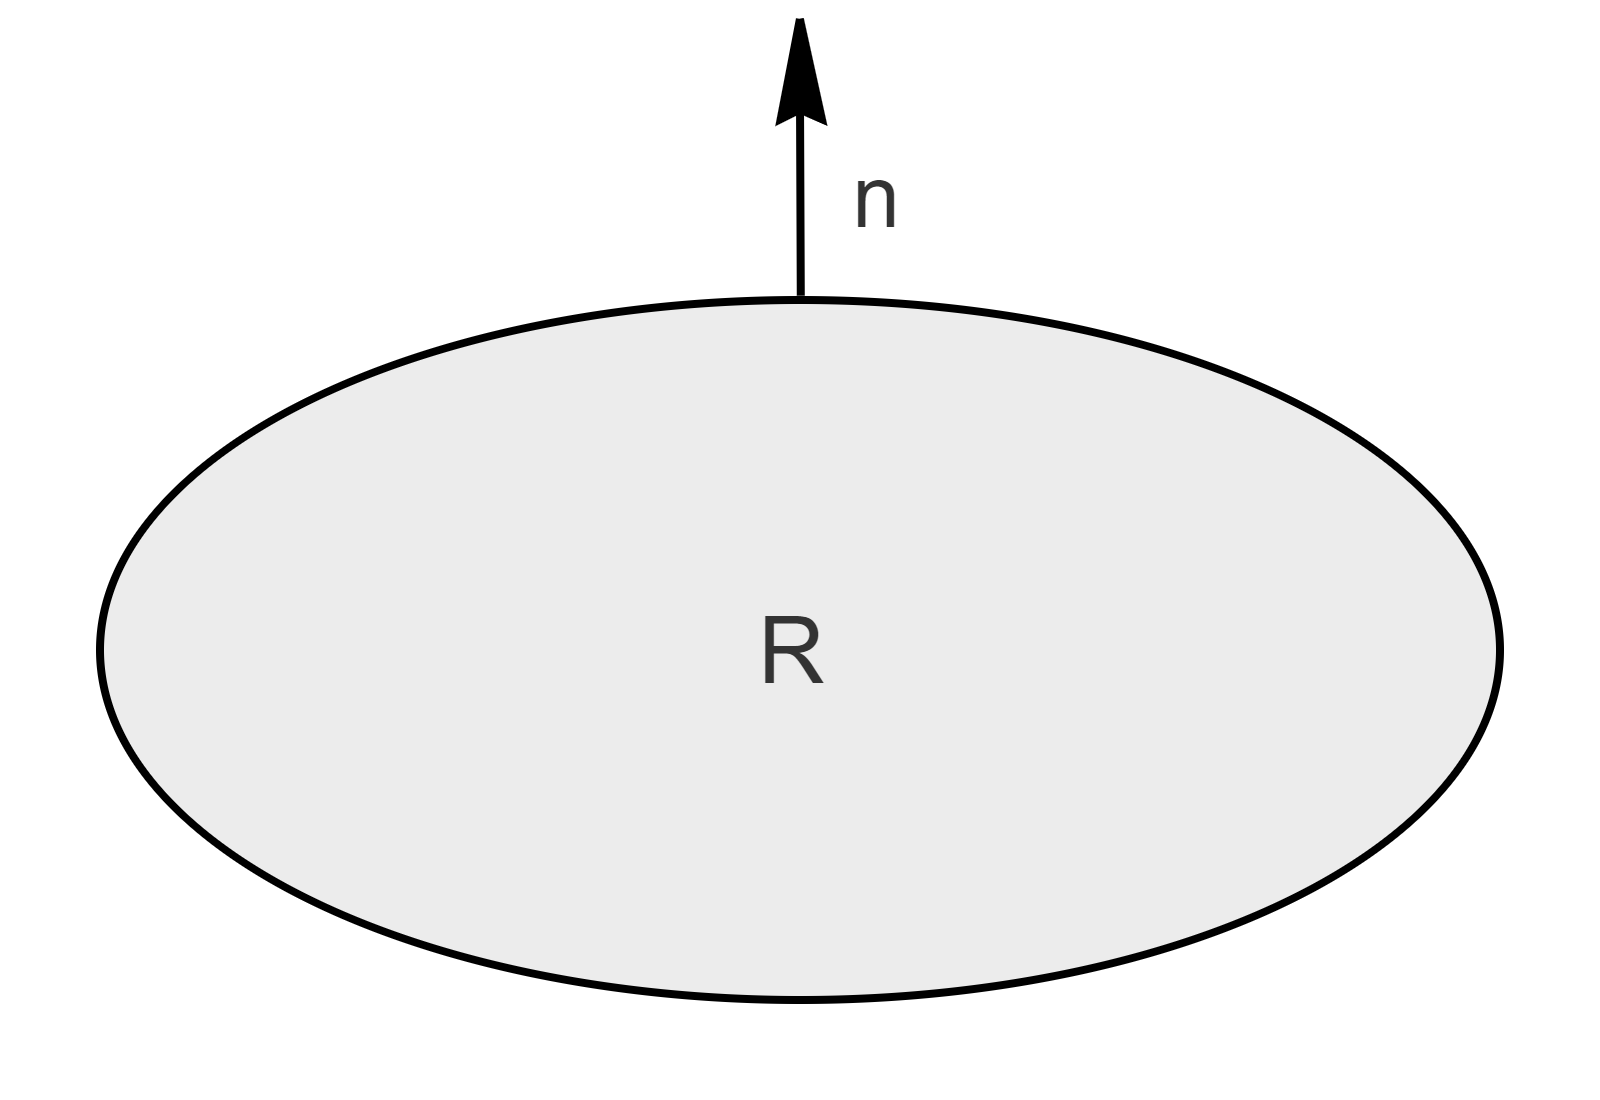
\includegraphics{pictures/normal_vector.png}
            }
        };
        \node at (0.4, 1.8) {$\mathbf{n}$};
        \node at (0, -0.5) {$R$};
    \end{tikzpicture}
    \centering 
    \caption{The region $R$ and its normal vector.} 
    \label{fig.normal_vector} 
\end{figure}

Before we introduce the concept of boundary conditions, let us first explain the concept of normal vectors.

\begin{definition}[Normal vector] Given a domain $R$ and a point $x\in \partial R$, a \underline{normal vector} $\mathbf{n}$ at $x$ is the vector as demonstrated by figure \ref{fig.normal_vector}. In this class, the normal vector is always pointing outwards. 
    
\end{definition}

Now we introduce the boundary conditions that will be considered in this class.

\begin{definition}[Boundary conditions] Consider a PDE $F[u] = 0$ defined on the domain $R$. Here are the boundary conditions that we consider in this class.
    \begin{enumerate}
        \item \textbf{Dirichlet boundary condition.} The value of $u$ on the boundary is given.
        \begin{equation}\label{eq.Dirichlet_boundary}
            u=g(x), \quad x \in \partial R .
        \end{equation}
        
        \item \textbf{Neumann boundary condition.} The normal derivative on the boundary is given.
        \begin{equation}\label{eq.Neumann_boundary}
            \mathbf{n} \cdot \nabla u=g(x), \quad x \in \partial R .
        \end{equation}
        
        \item \textbf{Robin boundary condition.} A linear combination of the above two boundary conditions. 
        \begin{equation}\label{eq.Robin_boundary}
            a(x) u+b(x) \mathbf{n} \cdot \nabla u=g(x), \quad x \in \partial R .
        \end{equation}
    \end{enumerate}
\end{definition}

\subsubsection{Heat equations as an example}

We take the heat equation $u_t = Ku_{zz}$, defined on $R = \{(z, t): 0 \le t < \infty,\ 0 \le x \le L\}$, as an example to explain these boundary conditions. 


The domain $R$ of the heat equation is described in the following picture,

\begin{figure}[H]
    \begin{tikzpicture}
        \node at (0, 0) {\scalebox{0.15}{      
            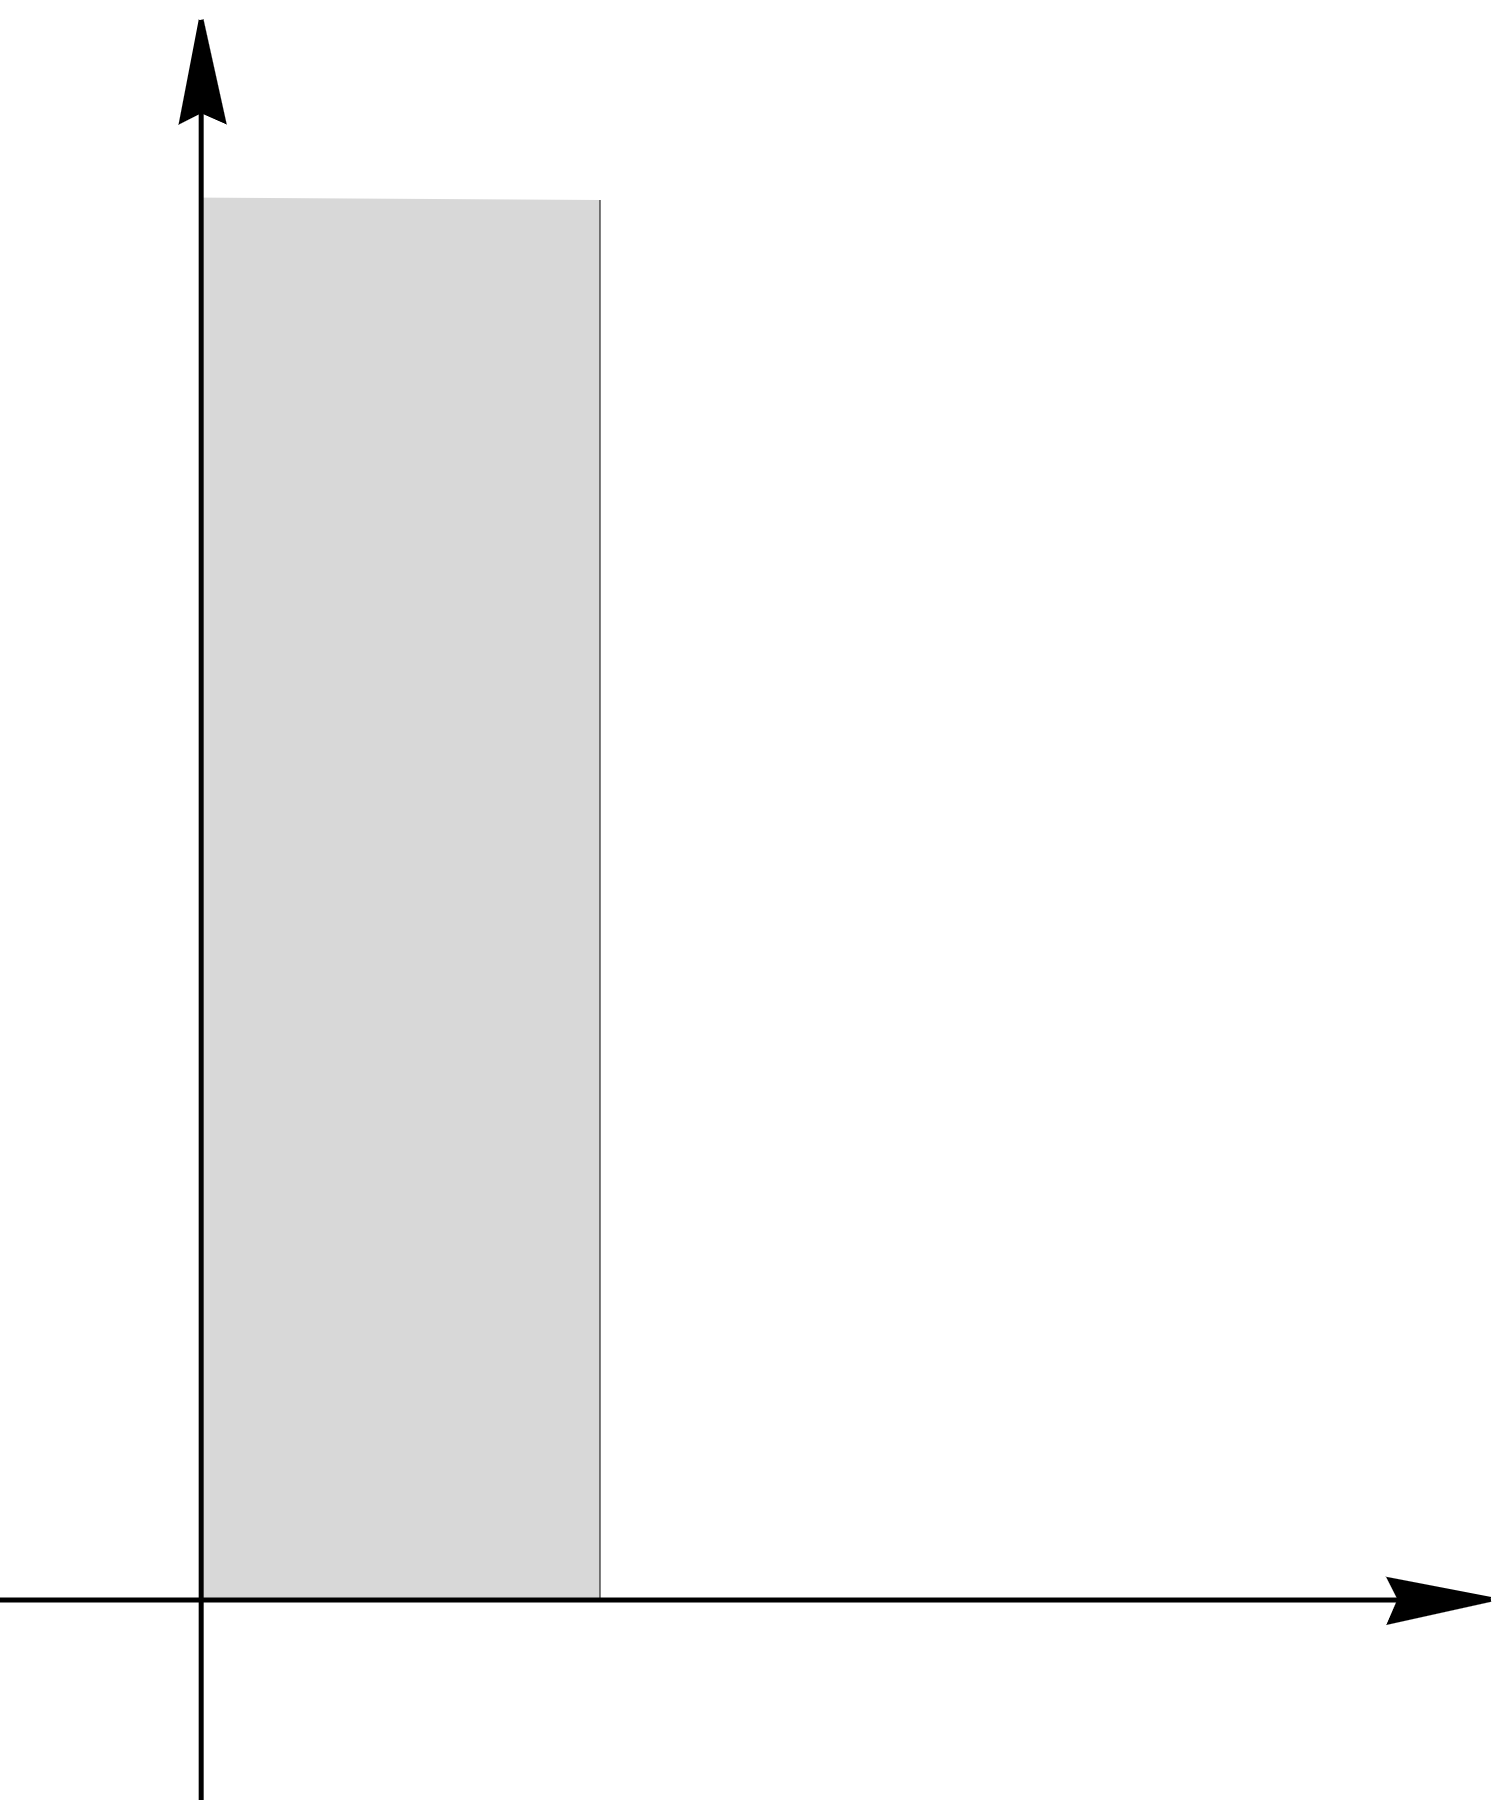
\includegraphics{pictures/heat_region.png}
        }};
        \node at (2.8, -3) {$z$};
        \node at (-1.9, 3.3) {$t$};
        \node at (-0.55, -3) {$L$};
        \node at (-1.4, -3) {$t = 0$};
        \node at (-0.1, -1.3) {$z = L$};
        \node at (-2.7, -1.3) {$z = 0$};
        \node at (-2.5, 0.2) {$\mathbf{n}_2$};
        \node at (-0.2, 0.2) {$\mathbf{n}_1$};
        \node at (-1.4, 0.1) {$R$};
        \node (1) at (-0.72, 0) {};
        \node (2) at (0.3,0) {};
        \draw[-Stealth] (1) -- (2);

        \node (3) at (-2.05, 0) {};
        \node (4) at (-3.05,0) {};
        \draw[-Stealth] (3) -- (4);
    \end{tikzpicture}
    \centering 
    \caption{The domain for the heat equation.} 
    \label{fig.heat_region} 
\end{figure}

There are three pieces of $\partial R$, 
\begin{equation}\label{eq.heat_boundary_3_pieces}
    \begin{split}
        &z=0, \quad t>0
        \\
        &z=L, \quad t>0
        \\
        &0<z<L, \quad t=0
    \end{split}
\end{equation}

On the first two parts of $\partial R$ corresponding to $z = 0,\, L$, we impose the Robin boundary condition. On the last part corresponding to $t = 0$, we impose the Dirichlet boundary condition. Then we get the following system of equations,
\begin{equation}\label{eq.heat_and_boundary_1}
    \left\{\begin{aligned} 
        &u_t=K u_{z z}, && 0<z<L, \quad t>0, 
        \\ 
        &a(z, t) u+b(z, t) \mathbf{n} \cdot \nabla u=g(z, t),\quad && z=0,\, L, \quad t>0, 
        \\
        &u(z, 0)=f(z), && 0<z<L, \quad t=0.
    \end{aligned}\right.
\end{equation}
Here the choice of Dirichlet and Robin boundary condition comes from the physics of heat conduction. We will explain this in section \ref{sec.}.

\textbf{TODO: second order need one condition but first order need one}


Now we explain how to simplify the Robin boundary condition in \eqref{eq.heat_and_boundary_1}.

On $z = 0$, from figure \ref{fig.heat_region}, we know that the normal vector $\mathbf{n} = (-1, 0)$ and $\nabla u = (u_z, u_t)$, so we get $\mathbf{n}\cdot \nabla u = -u_z$. Therefore, $a(z, t) u+b(z, t) \mathbf{n} \cdot \nabla u=g(z, t)$ simplifies to 
\begin{equation}\label{eq.heat_and_boundary_2}
    a(0, t) u - b(0, t) u_z = g(0, t).
\end{equation}

On $z = L$, from figure \ref{fig.heat_region}, we know that the normal vector $\mathbf{n} = (1, 0)$ and $\nabla u = (u_z, u_t)$, so we get $\mathbf{n}\cdot \nabla u = u_z$. Therefore, $a(z, t) u+b(z, t) \mathbf{n} \cdot \nabla u=g(z, t)$ simplifies to 
\begin{equation}\label{eq.heat_and_boundary_3}
    a(L, t) u + b(L, t) u_z = g(L, t).
\end{equation}

We introduce new functions $a(t)$, $\widetilde{a}(t)$, $b(t)$, $\widetilde{b}(t)$, $g(t)$ and $\widetilde{g}(t)$ by the following equations
\begin{equation}\label{eq.heat_and_boundary_4}
    \begin{split}
        &a(t) = a(0, t),\quad b(t) = b(0, t),\quad g(t) = g(0, t)
        \\
        &\widetilde{a}(t) = a(L, t),\quad \widetilde{b}(t) = b(L, t),\quad \widetilde{g}(t) = g(L, t)
    \end{split}
\end{equation}

Then the Robin boundary condition becomes
\begin{equation}\label{eq.heat_and_boundary_5}
    \begin{split}
        &a(t) u - b(t) u_z = g(t), \quad z = 0
        \\
        &\widetilde{a}(t) u + \widetilde{b}(t) u_z = \widetilde{g}(t), \quad z = L
    \end{split}
\end{equation}

The heat equation becomes
\begin{equation}\label{eq.heat_and_boundary_general}
    \left\{\begin{aligned} 
        &u_t=K u_{z z}, && 0<z<L, \quad t>0, 
        \\ 
        &a(t) u - b(t) u_z = g(t),\quad && z=0, \quad t>0, 
        \\ 
        &\widetilde{a}(t) u + \widetilde{b}(t) u_z = \widetilde{g}(t), && z=L, \quad t>0, 
        \\
        &u=f(z), && 0<z<L, \quad t=0.
    \end{aligned}\right.
\end{equation}

In order to make \eqref{eq.heat_and_boundary_general} solvable, we impose the homogeneous condition. 


\begin{definition}[Homogeneous] We say \eqref{eq.heat_and_boundary_general} is \underline{homogeneous} if 
    \begin{enumerate}
        \item $a(t)$, $\widetilde{a}(t)$, $b(t)$, $\widetilde{b}(t)$, $g(t)$ and $\widetilde{g}(t)$ are independent of $t$.
        \item $g(t) = \widetilde{g}(t) = 0$.
    \end{enumerate}
\end{definition}

With homogeneous assumption, \eqref{eq.heat_and_boundary_general} becomes
\begin{equation}\label{eq.heat_and_boundary_6}
    \left\{\begin{aligned} 
        &u_t=K u_{z z}, && 0<z<L, \quad t>0, 
        \\ 
        &a u - b u_z = 0,\quad && z=0, \quad t>0, 
        \\ 
        &\widetilde{a} u + \widetilde{b} u_z = 0, && z=L, \quad t>0, 
        \\
        &u=f(z), && 0<z<L, \quad t=0.
    \end{aligned}\right.
\end{equation}

To further simplify the above equation, we did the change of variable 
\begin{equation}
    b\rightarrow bL,\quad \widetilde{b}\rightarrow \widetilde{b}L
\end{equation}
followed by the change of variable
\begin{equation}
    \begin{split}
        &a\rightarrow r\cos \alpha,\quad b\rightarrow r\sin \alpha,
        \\
        &\widetilde{a}\rightarrow r\cos \beta,\quad \widetilde{b}\rightarrow r\sin \beta.
    \end{split}
\end{equation}

Finally, the heat equation becomes
\begin{equation}\label{eq.heat_and_boundary}
    \left\{\begin{aligned} 
        &u_t=K u_{z z}, && 0<z<L, \quad t>0, 
        \\ 
        &u \cos \alpha-L u_z \sin \alpha=0,\quad && z=0, \quad t>0, 
        \\ 
        &u \cos \beta+L u_z \sin \beta=0, && z=L, \quad t>0, 
        \\
        &u=f(z), && 0<z<L, \quad t=0,
    \end{aligned}\right.
\end{equation}


\subsubsection{Separation of variable in heat equation}

Let us solve the heat equation in a simple case of $\alpha=\beta=0$ in \eqref{eq.heat_and_boundary}. The separated solution is written as $u(z, t)=\phi(z) T(t)$. Thus we obtain
$$
T^{\prime}(t)+\lambda K T(t)=0, \quad \phi^{\prime \prime}(z)+\lambda \phi(z)=0 .
$$

The boundary conditions are written as
$$
\phi(0)=\phi(L)=0 .
$$

We obtain
$$
T(t)=e^{-\lambda K t}, \quad \phi=A \sin (\sqrt{\lambda} z)+B \cos (\sqrt{\lambda} z), \quad \lambda>0 .
$$

By plugging $\phi=A \sin (\sqrt{\lambda} z)+B \cos (\sqrt{\lambda} z)$ into the boundary conditions, we find that $B=0$ and $\sqrt{\lambda} L = n\pi$ where $n$ is an integer. Therefore we obtain
$$
\phi(z)=\phi_n(z)=\sin \left(\sqrt{\lambda_n} z\right), \quad \lambda_n=\left(\frac{n \pi}{L}\right)^2, \quad n=1,2, \ldots,
$$
where we set the arbitrary constant in $\phi_n(z)$ to be $1$ (recall we will take a superposition). Thus the separated solutions are obtained as
$$
u(z, t)=\phi_n(z) e^{-\lambda_n K t}, \quad n=1,2, \ldots
$$

If no initial condition $u(z, 0) = f(z)$ is given, the separated solutions are the solutions to the problem. However, they do not satisfies $u(z, 0) = f(z)$.
Let us consider the linear combination of separated solution and match with the initial condition.

The linear combination is 
$$
u(z, t)=\sum_{n=1}^{\infty} C_n \phi_n(z) e^{-\lambda_n K t},
$$
where $C_n$ are constants. 

By $u(z, 0) = f(z)$, we know that 

$$
f(z) = u(z, 0) = \sum_{n=1}^{\infty} C_n \phi_n(z) = \sum_{n=1}^{\infty} C_n \sin \frac{n\pi z}{L}.
$$

From this, we know that $C_n$ is the $B_n$ coefficient of the Fourier sine series. We thus obtain
$$
u(z, t)=\sum_{n=1}^{\infty} B_n \phi_n(z) e^{-\lambda_n K t}, \quad 0<z<L, \quad t>0 .
$$
$$
B_n=\frac{2}{L} \int_0^L f(x) \sin \frac{n \pi x}{L} d x.
$$

\begin{example}[]
The heat equation $u_t=K u_{z z}$ for $0<z<L, t>0$ with $u(0, t)=u(L, t)=0$ and $u(z, 0)=1$ is solved as
$$
u(z, t)=\sum_{n=1}^{\infty} B_n \sin \frac{n \pi z}{L} e^{-(n \pi / L)^2 K t},
$$
where  
$$
B_n=\frac{2}{\pi} \frac{1-(-1)^n}{n} .
$$

Here as mentioned above, $B_n$ can be directly computed as coefficients of the Fourier sine series of $f(z) = 1$
\end{example}

\subsubsection{Some linear algebra}

After the separation of the variable in the heat equation, we obtain the following equation
$$
\phi^{\prime \prime}(z)+\lambda \phi(z)=0 \quad \Leftrightarrow \quad -\phi^{\prime \prime}(z) = \lambda \phi(z).
$$

If we denote the negative second-order derivative operator by $A$, then we get
$$
A\phi = \lambda\phi.
$$ 

This is very similar to the eigenvalue and eigenvector equation for matrix $M$ in linear algebra.
\begin{equation}\label{eq.eigenvalue_linear_alg}
    M v = \lambda v.
\end{equation}

For a symmetric matrix, we have the following properties.

\begin{theorem}[]\label{th.SL_1_linear_alg} Assume that $M$ is a symmetric operator $(M = M^{T})$, and $\langle x, y\rangle$ is the inner product of vectors, then we have
\begin{enumerate}
    \item $\langle M x, y\rangle = \langle x, My\rangle$.
    \item The eigenvalues of $M$ are real numbers.
    \item If $v$, $w$ are eigenvectors with different eigenvalues $\lambda$ and $\mu$ respectively, then $v\perp w$ $(\langle v, w\rangle = 0)$.
\end{enumerate}
\end{theorem}
\begin{proof}
    Notice that $\langle x, y\rangle = x^T y$, then we have $\langle M x, y\rangle = (M x)^T y = x^T M^T y = x^T M y = \langle x, My\rangle$.

    For complex vectors $\langle x, y\rangle = \bar{x}^T y$, $\langle x, M x\rangle = \lambda\langle x, x\rangle$, $\langle M x, x\rangle = \bar{\lambda}\langle x, x\rangle$ and $\langle M x, x\rangle = \langle x, Mx\rangle$. Therefore, $\lambda = \bar{\lambda}$. 

    $\langle v, M w\rangle = \mu\langle v, w\rangle$, $\langle M v, w\rangle = \lambda\langle v, w\rangle$ and $\langle M v, w\rangle = \langle v, Mw\rangle$. Therefore, $\mu\langle v, w\rangle = \lambda \langle v, w\rangle$, which implies that $\langle v, w\rangle$ due to $\lambda\neq\mu$.
\end{proof}


It turns out that $A$ can be viewed as a symmetric matrix, and thus satisfies all properties described by Theorem \ref{th.SL_1_linear_alg}.


\subsection{The Sturm-Liouville eigenvalue problem}

Now we study the eigenvalue problems for differential operators. Let us first start with the concepts of orthogonal functions and symmetric operators. \textbf{TODO: we encounter so much orthogonality, which looks like a magic, explain the source of orthogonality}

\subsubsection{Orthogonal functions and symmetric operators}

\begin{definition}[Inner product] We extend dot product $\varphi \cdot \psi$ and define \underline{inner product} as
\begin{equation}\label{eq.inner_product}
    \langle\varphi, \psi\rangle=\int_a^b \varphi(x) \psi(x) d x .
\end{equation}
    
Sometimes the inner product is defined as follows. We can have a \underline{weight function} $\rho(x)$, and the weighted inner product is given by
\begin{equation}\label{eq.inner_product_weight}
    \langle\varphi, \psi\rangle_\rho=\int_a^b \varphi(x) \psi(x) \rho(x) d x
\end{equation}
where $\rho(x)>0$ is a weight function. 

For complex functions, we can write the \underline{complex inner product} as
\begin{equation}\label{eq.inner_product_complex}
    \langle\varphi, \psi\rangle=\int_a^b \varphi(x) \bar{\psi}(x) \rho(x) d x .
\end{equation}
Here $\bar{\psi}$ is the complex conjugate of $\psi$ $(\bar{\psi}(x)=f(x)-i g(x)$ when $\psi=f+i g)$.
    
\end{definition}

\begin{definition}[Orthogonality]
Two functions $\varphi, \psi$ are said to be \underline{orthogonal} on $[a, b]$ if $\langle\varphi, \psi\rangle=0$.    
\end{definition}

\begin{example}[]
    The functions $\varphi(x)=\sin x$ and $\psi(x)=\cos x$ are orthogonal on $[0, \pi]$.
\end{example}
\begin{example}[]
    The set of functions $1, \cos \frac{\pi x}{L}, \sin \frac{\pi x}{L}, \ldots, \cos \frac{N\pi x}{L}, \sin \frac{N\pi x}{L}$ is orthogonal on $[-L, L]$.
\end{example}

\begin{example}[]
    The set of functions $\{e^{\frac{in\pi x}{L}}\}_{n\in\mathbb{Z}}$ is orthogonal on $[-L, L]$.
\end{example}

\begin{example}[]
    Which of the following pairs of functions are orthogonal on the interval $0 \leq x \leq 1$?
$$
\varphi_1=\sin 2 \pi x, \quad \varphi_2=x, \quad \varphi_3=\cos 2 \pi x, \quad \varphi_4=1 .
$$
$\left\langle\varphi_1, \varphi_3\right\rangle=0,\left\langle\varphi_1, \varphi_4\right\rangle=0,\left\langle\varphi_2, \varphi_3\right\rangle=0,\left\langle\varphi_3, \varphi_4\right\rangle=0$. All others are nonzero. Therefore the pairs $\left(\varphi_1, \varphi_3\right),\left(\varphi_1, \varphi_4\right),\left(\varphi_2, \varphi_3\right)$, and $\left(\varphi_3, \varphi_4\right)$ are orthogonal.
\end{example}

\begin{definition}[Norm]
As follows we define \underline{norm}, which is the ``length'' of a function.
$$
\|\varphi\|=\|\varphi\|_{L^2(a, b)}=\sqrt{\langle\varphi, \varphi\rangle} .
$$
We note that the norm is always nonnegative. The norm $\|\varphi-\psi\|$ is the distance between two functions $\varphi$ and $\psi$.
\end{definition}

\begin{definition}[Orthonormal]
    The functions $\left(\varphi_1, \ldots, \varphi_N\right)$ are orthonormal if $\left\langle\varphi_i, \varphi_j\right\rangle=$ $\delta_{i j}$. Here $\delta_{i j}$ is the Kronecker delta $(\delta_{i j}=0$ if $i \neq j$ and $=1$ if $i=j)$.
\end{definition}

\begin{definition}[Normalization]
    Let $\{\varphi_1, \varphi_2, \ldots, \varphi_N\}$ be a set of orthogonal functions satisfying $\varphi_i \perp \varphi_j$ for $i \neq j$. Each function $\varphi_i$ can be \underline{normalized} to obtain an orthogonal sequence $\{\psi_i\}_{i = 1, \dots, N}$:
    \[
    \psi_i = \frac{\varphi_i}{\|\varphi_i\|}
    \]
    where $\|\varphi_i\|$ denotes the norm of the function $\varphi_i$.
    
\end{definition}

\begin{example}[]
    After normalize the orthogonal functions $\cos x$, $\sin x$ on $[0, \pi]$, we obtain $\sqrt{\frac{2}{\pi}}\cos x$, $\sqrt{\frac{2}{\pi}}\sin x$.
\end{example}

\begin{definition}[Differential Operator]
    A \underline{differential operator} $A$ is an operator satisfying the following
    \begin{enumerate}
        \item $A$ is of the form $A = \sum_{i=0}^{n} a_i(x) \frac{d^i}{dx^i}$.
        \item The operator $A$ has a domain $\mathrm{Dom}(A)$, which means that $A$ does accept all smooth functions as its input. (See Example \ref{ex.symm_op} for an example of $\mathrm{Dom}(A)$)
    \end{enumerate}  
    \noindent where $n$ is a non-negative integer representing the \underline{order} of the differential operator, $a_i(x)$ are the \underline{coefficient} of $A$, and $\frac{d^i}{dx^i}$ represents the $i$-th derivative with respect to $x$, with $\frac{d^0}{dx^0}$ interpreted as the identity operator.

\end{definition}

\begin{definition}[Symmetric operators] Given a differential operator $A$, we say $A$ is \underline{symmetric}, if for any functions $\varphi, \psi\in \mathrm{Dom}(A)$,
\begin{equation}\label{eq.symm_operator}
    \langle A\varphi, \psi\rangle = \langle \varphi, A\psi\rangle.
\end{equation}
    
\end{definition}

\begin{example}[]\label{ex.symm_op}
The differential operator $A$ defined by the following is a symmetric operator,
\begin{equation}
A = -\frac{d^2}{dx^2},\qquad \mathrm{Dom}(A) = \{\varphi(x): x\in [a, b],\,\varphi(a) = \varphi(b) = 0\}
\end{equation}

To show that $A$ is symmetric, we need to verify that
\begin{equation}\label{eq.ex_symm_op_1}
\langle \varphi, A\psi \rangle = \langle A\varphi, \psi \rangle
\end{equation}
for all functions $\varphi(x)$ and $\psi(x)$ satisfying $\varphi(a) = \varphi(b) = \psi(a) = \psi(b) = 0$. This condition translates into the following integral equality,
\begin{equation}
\int_a^b \varphi(x) \psi''(x) dx = \int_a^b \varphi''(x) \psi(x) dx
\end{equation}
Applying integration by parts and using the boundary conditions $\varphi(a) = \varphi(b) = \psi(a) = \psi(b) = 0$, we get
\begin{equation}
\begin{split}
    \int_a^b \varphi''(x) \psi(x) dx =& \underbrace{\left[\varphi'(x) \psi(x)\right]_a^b}_{ = 0} - \int_a^b \varphi'(x) \psi'(x) dx 
    \\
    =& - \int_a^b \varphi'(x) \psi'(x) dx = -\underbrace{\left[\varphi(x) \psi'(x)\right]_a^b}_{ = 0} + \int_a^b \varphi(x) \psi''(x) dx
    \\
    =& \int_a^b \varphi(x) \psi''(x) dx
\end{split}
\end{equation}
This equality confirms \eqref{eq.ex_symm_op_1} and thus the fact that $A$ is symmetric on the given domain $\mathrm{Dom}(A)$.
\end{example}

\begin{example}
    The definition of symmetric operator depends on domain. For example, if we define $A$ by 
    \begin{equation}
        A = -\frac{d^2}{dx^2},\qquad \mathrm{Dom}(A) = \{\varphi(x): x\in [a, b]\}
    \end{equation}
    which is almost the same operator as the last example but with a different domain. This operator is NOT symmetric. If we take $\varphi(x) = 1$ and $\psi(x) = x$, then a straightforward computation gives $\langle \varphi, A\psi \rangle = 0$ and  $\langle A\varphi, \psi \rangle \neq 0$. Therefore, $A$ is not symmetric.
\end{example}

% \begin{definition}[Projection]
%     Let $\left(\varphi_1, \ldots, \varphi_N\right)$ be a set of orthogonal functions with $\left\|\varphi_i\right\| \neq 0$. Let $f(x)$ be a function. Then $\hat{c}_1 \varphi_1+\cdots+\hat{c}_N \varphi_N$ with $\hat{c}_i=$ $\left\langle f, \varphi_i\right\rangle /\left\|\varphi_i\right\|^2$ is the projection of $f$ onto $\left(\varphi_1, \ldots, \varphi_N\right) . \hat{c}_i$ is called the $i$ th Fourier coefficient of $f$. 

%     \textbf{TODO: revise this}
% \end{definition}


% Note that the minimum of $\left\|f-\left(c_1 \varphi_1+\cdots+c_N \varphi_N\right)\right\|$ is achieved when $c_i=\hat{c}_i$.

% \begin{example}[]
%     Find the projection of $f(x)=1$ onto $\left(\varphi_1, \varphi_2\right)=(\sin x, \sin 2 x)$ on the interval $0 \leq x \leq \pi$. By $\left\langle f, \varphi_1\right\rangle=2,\left\langle f, \varphi_2\right\rangle=0$, and $\left\|\varphi_1\right\|^2=\left\|\varphi_2\right\|^2=\frac{\pi}{2}$, we obtain $\frac{4}{\pi} \sin x$.   
% \end{example}

\subsubsection{The Sturm-Liouville eigenvalue problem}\label{sec.Sturm_Liouville}

\begin{definition}[Sturm-Liouville problems]
Let $\phi$ be a function defined on the interval $(a, b)$, the \underline{Sturm-Liouville problems} is the following boundary value problem,
\begin{equation}\label{eq.Sturm_Liouville}
    \begin{split}
        &\left[s(x) \phi^{\prime}(x)\right]^{\prime}+[\lambda \rho(x)-q(x)] \phi(x)=0, \quad a<x<b,
        \\
        &\ \phi(a) \cos \alpha-L \phi^{\prime}(a) \sin \alpha=0,
        \\
        &\ \phi(b) \cos \beta+L \phi^{\prime}(b) \sin \beta=0
    \end{split}
\end{equation}
where $\rho$ is a positive function $\rho(x)>0$ and $L=b-a$, $\alpha, \beta \in[0, \pi)$ are some parameters. 
\end{definition}

Define the operator $A$ by 
\begin{equation}\label{eq.A_op_Sturm_Liouville}
    A \phi = - \frac{1}{\rho(x)}\left(\left[s(x) \phi^{\prime}(x)\right]^{\prime}-q(x) \phi(x)\right)
\end{equation}
with domain
\begin{equation}\label{eq.A_op_Sturm_Liouville_dom}
    \left\{\phi(x),\, x\in [a, b]\,\Bigg|\begin{aligned}
        &\ \phi(a) \cos \alpha-L \phi^{\prime}(a) \sin \alpha=0,
        \\
        &\ \phi(b) \cos \beta+L \phi^{\prime}(b) \sin \beta=0
    \end{aligned}
    \right\}
\end{equation}
then \eqref{eq.Sturm_Liouville} is equivalent to
\begin{equation}\label{eq.Sturm_Liouville'}
    A \phi = \lambda \phi.
\end{equation}


The following theorem claims that all symmetric second order differential operators are of the form given by \eqref{eq.A_op_Sturm_Liouville} and \eqref{eq.A_op_Sturm_Liouville_dom}.

\begin{theorem}
    A symmetric second order differential operator $A$ must be of the form given by \eqref{eq.A_op_Sturm_Liouville} and \eqref{eq.A_op_Sturm_Liouville_dom}.
\end{theorem}
\begin{proof}
    The proof go beyond the scope of this course.
\end{proof}

The following theorem explain the procedure of reducing an arbitrary second order differential operator to a Sturm-Liouville operator. Since it is abstract, it is good to first jump to the examples below the theorem.
\begin{theorem}[]\label{th.reduction_to_SL}
    Given an arbitrary second order linear differential equation $a(x)y'' + b(x)y' + c(x)y = 0$, it can be reduced to the Sturm-Liouville equation \eqref{eq.Sturm_Liouville} by the following procedure.
    \begin{enumerate}
        \item Divide both sides by $a(x)$ to obtain $y'' + p(x)y' + q(x)y = 0$.
        \item Solve the equation $\widehat{y}' = p(x)\widehat{y}$.
        \item Multiply both sides of $y'' + p(x)y' + q(x)y = 0$ by $\widehat{y}$
        \begin{equation}
            \widehat{y}(y'' + p(x)y') + \widehat{y}q(x)y = 0\quad \Rightarrow\quad (\widehat{y}y')' + \widehat{y}q(x)y = 0
        \end{equation}
    \end{enumerate}
\end{theorem}
\begin{proof}
    There is nothing to prove.
\end{proof}

\begin{example}[Bessel functions] The \underline{Bessel functions} are solutions of the following ODEs.
\begin{equation}\label{eq.Bessel}
    \phi^{\prime \prime}+(d-1) \frac{\phi^{\prime}}{x}+\left(1-\frac{\mu}{x^2}\right) \phi=0.
\end{equation}
We can apply the procedure in Theorem \ref{th.reduction_to_SL} to reduce the above equation to a Sturm-Liouville equation.

\begin{enumerate}
    \item There is nothing to do with this step since $a(x) = 1$.
    \item We first solve $\widehat{y}' = \frac{d-1}{x}\widehat{y}$ and obtain $\widehat{y}(x) = x^{d-1}$.
    \item Multiply both side of $\phi^{\prime \prime}+(d-1) \frac{\phi^{\prime}}{x}+\left(1-\frac{\mu}{x^2}\right) \phi=0$ by $x^{d-1}$, then we get 
    \begin{equation}
        x^{d-1}\cdot\left(\phi^{\prime \prime}+(d-1) \frac{\phi^{\prime}}{x}+\left(1-\frac{\mu}{x^2}\right) \phi\right)=0 \quad \Rightarrow\quad (x^{d-1}\phi')'+\left(x^{d-1}-\mu x^{d-3}\right) \phi=0.
    \end{equation}
\end{enumerate}
Finally, we get
\begin{equation}\label{eq.Bessel_SL}
    (x^{d-1}\phi'(x))'+\left(x^{d-1}-\mu x^{d-3}\right) \phi(x)=0.
\end{equation}
This is a Sturm-Liouville equation by setting $s(x)=\rho(x)=x^{d-1}$, $q(x)=\mu x^{d-3}$, and $\lambda=1$.

In the case of $d=2$ and $\mu=m^2$ with $m\in \mathbb{N}$, the function $\phi(x)=J_m(x)$ is called the \underline{standard Bessel function}. In the case of $d=3$ and $\mu=k(k+1)(k=0,1,2, \ldots)$, the function $\phi(x)=j_k(x)$ is called the \underline{spherical Bessel function}.
\end{example}

\begin{example}[Legendre polynomials] The \underline{Legendre polynomials} $P_k^m(x)$ are solutions of the following ODEs.
    \begin{equation}\label{eq.Legendre}
        (1-x^2) \phi^{\prime \prime}-2 x \phi^{\prime}+\left(k(k+1)-\frac{m^2}{1-x^2}\right) \phi=0.
    \end{equation}
    We can apply the procedure in Theorem \ref{th.reduction_to_SL} to reduce the above equation to a Sturm-Liouville equation.
    
    \begin{enumerate}
        \item Divide both sides by $(1-x^2)$, then we get
        \begin{equation}\label{eq.ex_Legendre_1}
            \phi^{\prime \prime}-\frac{2x}{1-x^2} \phi^{\prime}+\left(\frac{k(k+1)}{1-x^2}-\frac{m^2}{(1-x^2)^2}\right) \phi=0 .
        \end{equation}
        \item We first solve $\widehat{y}' = -\frac{2x}{1-x^2}\widehat{y}$ and obtain $\widehat{y}(x) = 1-x^2$.
        \item Multiply both side $1-x^2$ (This step undo the operation of step 1 which sometimes appears), then we get 
        \begin{equation}
            (1-x^2) \phi^{\prime \prime}-2 x \phi^{\prime}+\left(k(k+1)-\frac{m^2}{1-x^2}\right) \phi=0  \ \  \Rightarrow\ \ ((1-x^2) \phi')'+\left(k(k+1)-\frac{m^2}{1-x^2}\right) \phi=0 .
        \end{equation}
    \end{enumerate}
Finally, we get
\begin{equation}\label{eq.Legendre_SL}
    ((1-x^2) \phi')'+\left(k(k+1)-\frac{m^2}{1-x^2}\right) \phi=0.
\end{equation}
This is a Sturm-Liouville equation by setting $s(x)=1-x^2$, $\rho(x)=1$, $q(x)=m^2 / (1-x^2)$, and $\lambda=k(k+1)$ ($k=0,1,2, \ldots$) with $a=-1$ and $b=1$.
\end{example}

\begin{example}[Hermite polynomials] The \underline{Hermite polynomials} $H_n(x)$ are solutions of the following ODEs.
    \begin{equation}\label{eq.Hermite}
        \phi^{\prime \prime}-x \phi^{\prime}+n \phi=0 .
    \end{equation}
    We can apply the procedure in Theorem \ref{th.reduction_to_SL} to reduce the above equation to a Sturm-Liouville equation.
    
    \begin{enumerate}
        \item There is nothing to do with this step since $a(x) = 1$.
        \item We first solve $\widehat{y}' = -x\widehat{y}$ and obtain $\widehat{y}(x) = e^{-\frac{x^2}{2}}$.
        \item Multiply both side by $e^{-\frac{x^2}{2}}$, then we get 
        \begin{equation}
            e^{-\frac{x^2}{2}}(\phi^{\prime \prime}-x \phi^{\prime})+n e^{-\frac{x^2}{2}} \phi=0 \quad \Rightarrow\quad \left(e^{-\frac{x^2}{2}}\phi'\right)'+n e^{-\frac{x^2}{2}}\phi=0.
        \end{equation}
    \end{enumerate}
    Finally, we get
    \begin{equation}\label{eq.Hermite_SL}
        \left(e^{-\frac{x^2}{2}}\phi'\right)'+n e^{-\frac{x^2}{2}}\phi=0.
    \end{equation}
    This is a Sturm-Liouville equation by setting $s(x)=\rho(x)=\exp \left(-x^2 / 2\right)$, $q(x)=0$, $\lambda=n$ $(n=0,1,2, \ldots)$ with $a=-\infty$ and $b=\infty$.
\end{example}


\subsubsection{The Sturm-Liouville theorem}
Recall that the Sturm-Liouville problem is equivalent to the eigenvalue problem $A \phi = \lambda \phi$ of the operator $A$ defined in \eqref{eq.A_op_Sturm_Liouville} and \eqref{eq.A_op_Sturm_Liouville_dom}, which are copied below. 
\begin{equation}\label{eq.A_op_Sturm_Liouville'}
    A \phi = - \frac{1}{\rho(x)}\left(\left[s(x) \phi^{\prime}(x)\right]^{\prime}-q(x) \phi(x)\right)
\end{equation}
with domain
\begin{equation}\label{eq.A_op_Sturm_Liouville_dom'}
    \left\{\phi(x),\, x\in [a, b]\,\Bigg|\begin{aligned}
        &\ \phi(a) \cos \alpha-L \phi^{\prime}(a) \sin \alpha=0,
        \\
        &\ \phi(b) \cos \beta+L \phi^{\prime}(b) \sin \beta=0
    \end{aligned}
    \right\}
\end{equation}


We have the following theorem, which is an analog of Theorem \ref{th.SL_1_linear_alg}
\begin{theorem}[Sturm-Liouville theorem I]\label{th.SL_1} Assume that $A$ is a differential operator defined by \eqref{eq.A_op_Sturm_Liouville} and \eqref{eq.A_op_Sturm_Liouville_dom}, and $\langle\varphi, \psi\rangle_\rho=\int_a^b \varphi(x) \psi(x) \rho(x) dx$ is the inner product defined by \eqref{eq.inner_product_weight} , then we have
\begin{enumerate}
    \item $\langle A \phi, \psi\rangle = \langle \phi, A\psi\rangle$.
    \item The eigenvalues of $A$ are real numbers.
    \item If $\varphi$, $\psi$ are eigenfunctions with different eigenvalues $\lambda$ and $\mu$ respectively, then $\langle \varphi, \psi\rangle_\rho = 0$.
    \item Assume that $\{\lambda_1,\lambda_2,\dots\}$ are the set of all eigenfunctions of $A$, then this set is infinite and discrete. \textbf{TODO: picture}
\end{enumerate}
\end{theorem}
\begin{proof}
    1. $A$ is symmetric. Consider $\langle A\phi, \psi \rangle$, and apply integration by parts
    \begin{equation}\label{eq.proof_SL_integral_parts}
    \begin{split}
        \langle A\phi, \psi \rangle =& \int_a^b \left(-\frac{1}{\rho(x)}[(s(x)\phi'(x))' - q(x)\phi(x)]\right) \psi(x) \rho(x) \, dx. 
        \\
        =& \int_a^b \left( -(s(x)\phi'(x))' + q(x)\phi(x) \right)\psi(x) \, dx. 
        \\
        =&-[s(x)\phi'(x)\psi(x)]_a^b + \int_a^b s(x)\phi'(x)\psi'(x) \, dx - \int_a^b q(x)\phi(x)\psi(x) \, dx.
    \end{split} 
    \end{equation}

    Similarly for $\langle \phi, A\psi\rangle = \langle A\psi, \phi\rangle$, we also have
    \begin{equation}\label{eq.proof_SL_integral_parts'}
    \begin{split}
        \langle A\psi, \phi\rangle =& \int_a^b \left(-\frac{1}{\rho(x)}[(s(x)\psi'(x))' - q(x)\psi(x)]\right) \phi(x) \rho(x) \, dx. 
        \\
        =& \int_a^b \left( -(s(x)\psi'(x))' + q(x)\psi(x) \right)\phi(x) \, dx. 
        \\
        =&-[s(x)\psi'(x)\phi(x)]_a^b + \int_a^b s(x)\psi'(x)\phi'(x) \, dx - \int_a^b q(x)\psi(x)\phi(x) \, dx.
    \end{split} 
    \end{equation}
    
    It suffices to show that the boundary terms are equal
    \begin{equation}\label{eq.proof_SL_boundary}
        [s(x)\phi'(x)\psi(x)]_a^b = [s(x)\psi'(x)\phi(x)]_a^b
    \end{equation}

    \textbf{TODO: finish the proof}
    
    2.  The eigenvalues of $A$ are real. Since the eigenvalues and eigenfunctions at this point may not be real, we consider the complex inner product. Let $\lambda$ be an eigenvalue with eigenfunction $\phi$,
    \begin{equation}
    A\phi = \lambda \phi.
    \end{equation}
    
    Consider the inner product $\langle \phi, A\phi \rangle$ and $\langle A\phi, \phi \rangle$,
    \begin{equation}
    \langle A\phi, \phi \rangle =  \langle \lambda\phi, \phi \rangle = \lambda \|\phi\|^2.
    \end{equation}
    \begin{equation}
        \langle \phi, A\phi \rangle =  \langle \phi, \lambda\phi \rangle = \overline{\lambda} \|\phi\|^2.
    \end{equation}
    
    Since $A$ is symmetric, we have $\langle \phi, A\phi \rangle$ and $\langle A\phi, \phi \rangle$, which implies that
    \begin{equation}
    \lambda \|\phi\|^2 = \overline{\lambda} \|\phi\|^2.
    \end{equation}
    
    Hence, $\lambda = \overline{\lambda}$, implying that $\lambda$ is real.
    
    3. Orthogonality of eigenfunctions with different eigenvalues. Now the eigenvalues and eigenfunctions at this point are real, we consider the real inner product.
    
    Suppose $A\phi = \lambda \phi$ and $A\psi = \mu \psi$ with $\lambda \neq \mu$. Consider
    \begin{equation}
    \lambda \langle \phi, \psi \rangle = \langle A\phi, \psi \rangle = \langle \phi, A\psi \rangle = \mu \langle \phi, \psi \rangle.
    \end{equation}
    
    Thus, $(\lambda - \mu) \langle \phi, \psi \rangle = 0$, implying $\langle \phi, \psi \rangle = 0$ if $\lambda \neq \mu$.
    
    4. Discreteness of the eigenvalue set. 
    \textbf{TODO: finish the proof}
\end{proof}

\textbf{TODO: the following property are unique to SL problem, multiplicity 1}
\begin{theorem}[Sturm-Liouville theorem II]\label{th.SL_2} Assume that $A$ is a differential operator defined by \eqref{eq.A_op_Sturm_Liouville} and $\phi_1$ and $\phi_2$ are the eigenfunctions of the same eigenvalue $\lambda$, then we exists a constant $C$ such that 
    \begin{equation}\label{eq.SL_multiplicity_one}
        \phi_1(x) = C\phi_2(x).
    \end{equation}
\end{theorem}

\begin{proof}
We consider
$$
\psi(x)= \begin{cases}\phi_2(a) \phi_1(x)-\phi_1(a) \phi_2(x), & \text { if } \alpha \neq 0 \\ \phi_2^{\prime}(a) \phi_1(x)-\phi_1^{\prime}(a) \phi_2(x), & \text { if } \alpha=0 .\end{cases}
$$

This $\psi(x)$ obeys (2.8). We have $\psi(a)=0$. Also $\psi^{\prime}(a)=0$ by (2.7). Thus $\psi(x)$ is a solution to (2.8) with initial conditions $\psi(a)=\psi^{\prime}(a)=0$. We can conclude that $\psi(x)=0, a<x<b$. Therefore,
$$
\phi_2(x)=C \phi_1(x), \quad C=\frac{\phi_2(a)}{\phi_1(a)} \quad \text { or } \quad \frac{\phi_2^{\prime}(a)}{\phi_1^{\prime}(a)} .
$$

\end{proof}


\subsubsection{Convergence of orthogonal series}

\subsection{The heat equation}

\subsubsection{Physics of heat conduction}

\subsubsection{The homogeneous case}

\subsubsection{The non-homogeneous case}

\subsection{The wave equation}

\subsubsection{Physics of string vibration}

\subsubsection{The homogeneous case}

\subsubsection{The non-homogeneous case}


\subsection{The Laplace's equation}

\subsubsection{Physics of static electricity}

\subsubsection{The homogeneous case}

\subsubsection{The non-homogeneous case}